\documentclass[11pt,a4paper]{article}

\usepackage{amsmath}
\usepackage{graphicx}
\usepackage{epstopdf}

\title{AMTH250 \\ Assignment 4}

\author{Mark Villar}

\begin{document}

\maketitle

\subsubsection*{Question 1} Graph of $f(x)=(x-1)(x-3)$ over the interval $x \in [0,4]$, displaying the $x-$axis and its roots.
\begin{center}
	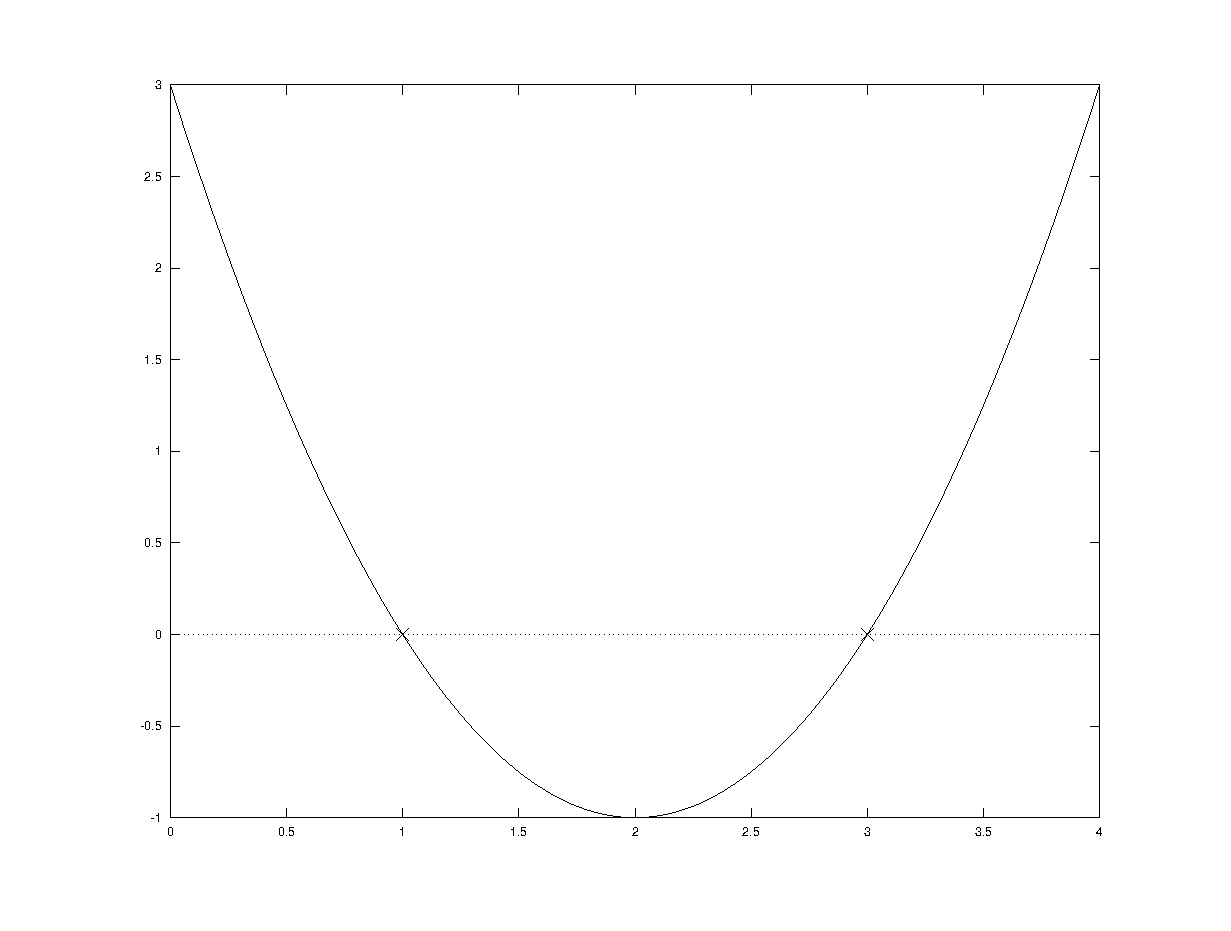
\includegraphics[width=1.1\textwidth]{plot1.eps}
\end{center}

\pagebreak

\subsubsection*{Question 2}
\begin{enumerate}

	\item[(a)] Graph of $f(x)=x\ln x$ over the interval $x \in [0,2]$.
	\begin{center}
		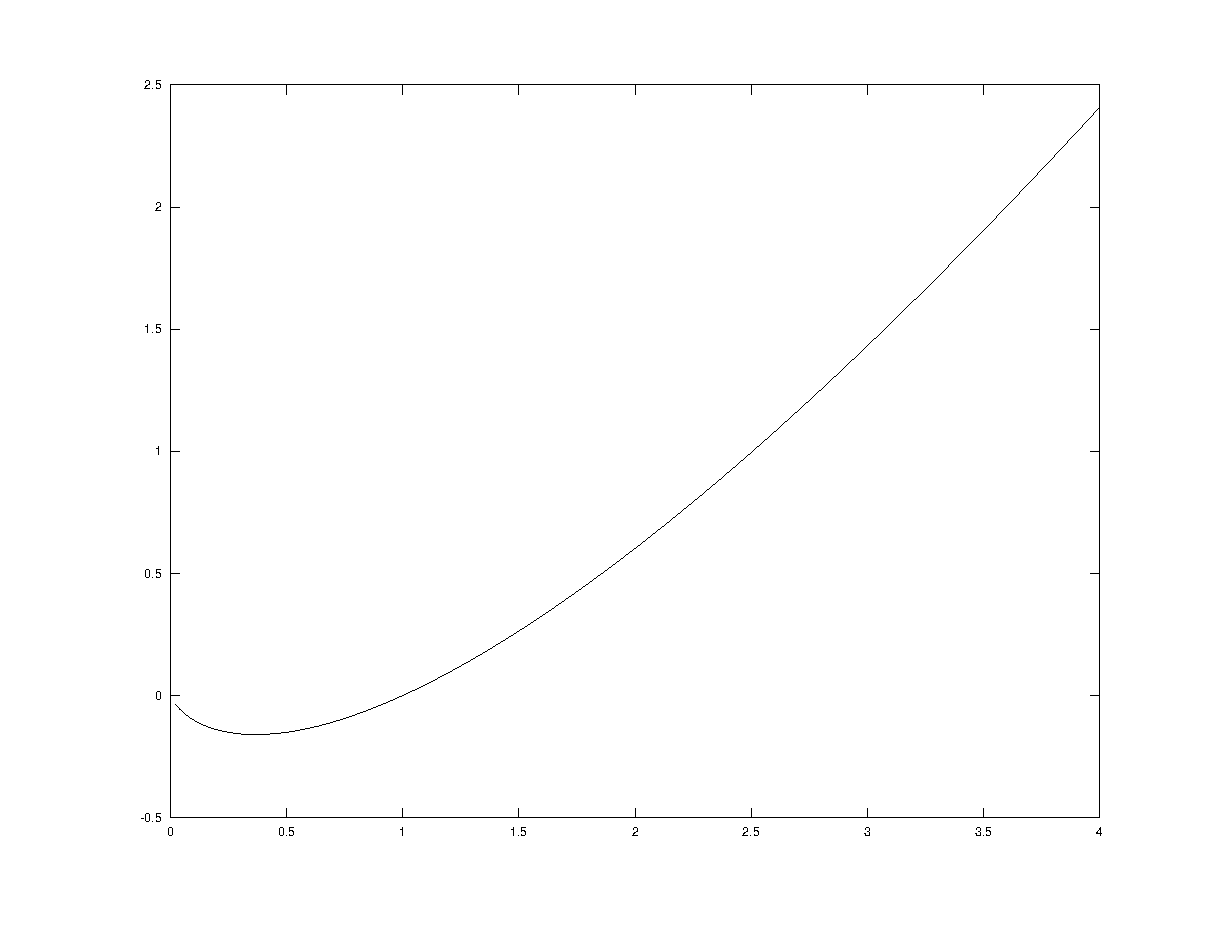
\includegraphics[width=0.9\textwidth]{plot2.eps}
	\end{center}
	
	\item[(b)] The curve approaches the origin from the right but never reaches it. This is because Octave evaluates $f(x)$ at $x=0$ as $f(0)= 0 \times (-\text{Inf})=$ NaN. To fix this, you could plot the graph of $f(x)$ over the interval $x \in (0,2]$ such that $x=0$ is excluded.
	
\end{enumerate}

\pagebreak

\subsubsection*{Question 3}

\begin{enumerate}

	\item[(a)] Graph of $f(x)=\frac{1}{1-x^2}$ over the interval $x \in [-2,2]$ with default scaling.
	\begin{center}
		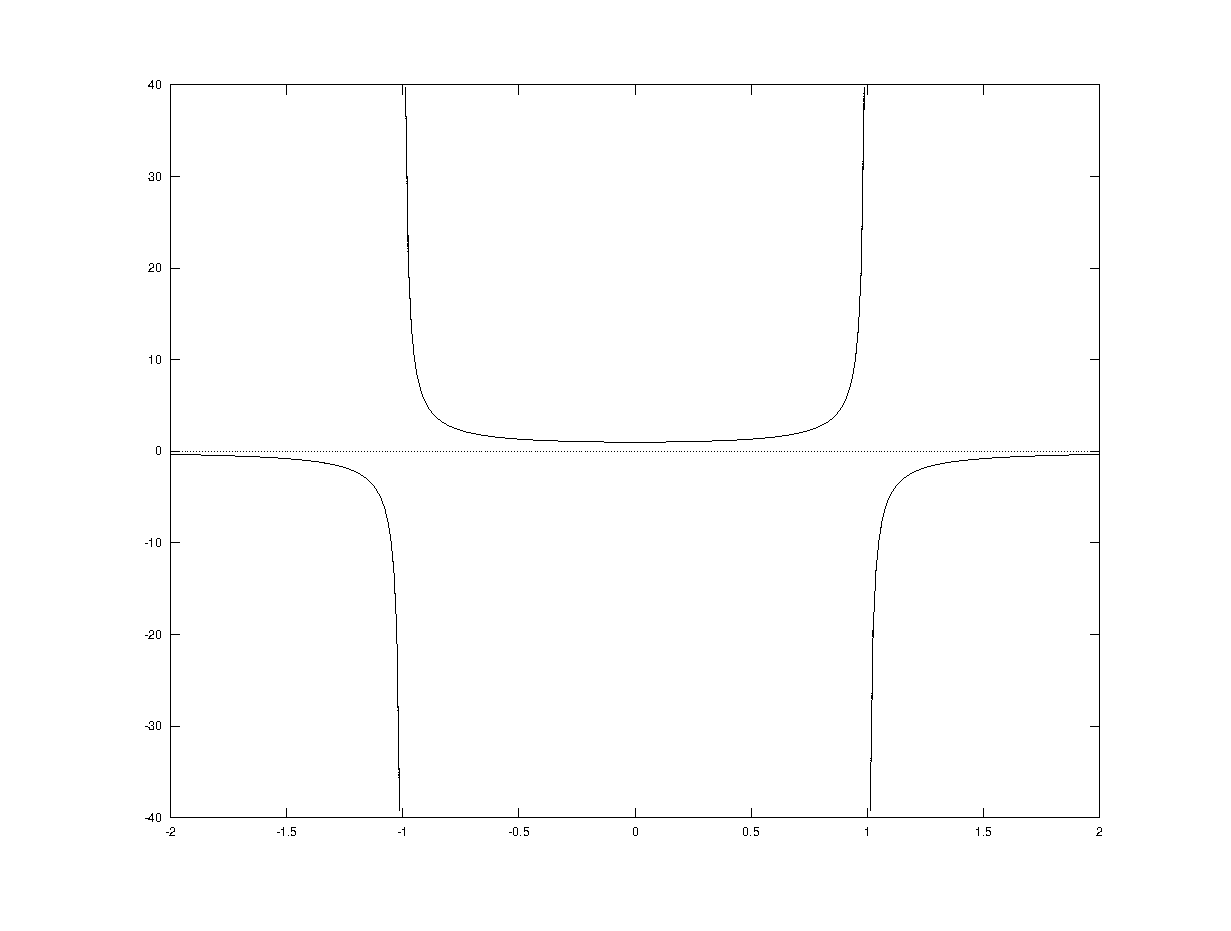
\includegraphics[width=0.8\textwidth]{plot3a.eps}
	\end{center}
	
	\item[(b)] Graph of $f(x)=\frac{1}{1-x^2}$ with rescaled $y$-axis.
	\begin{center}
		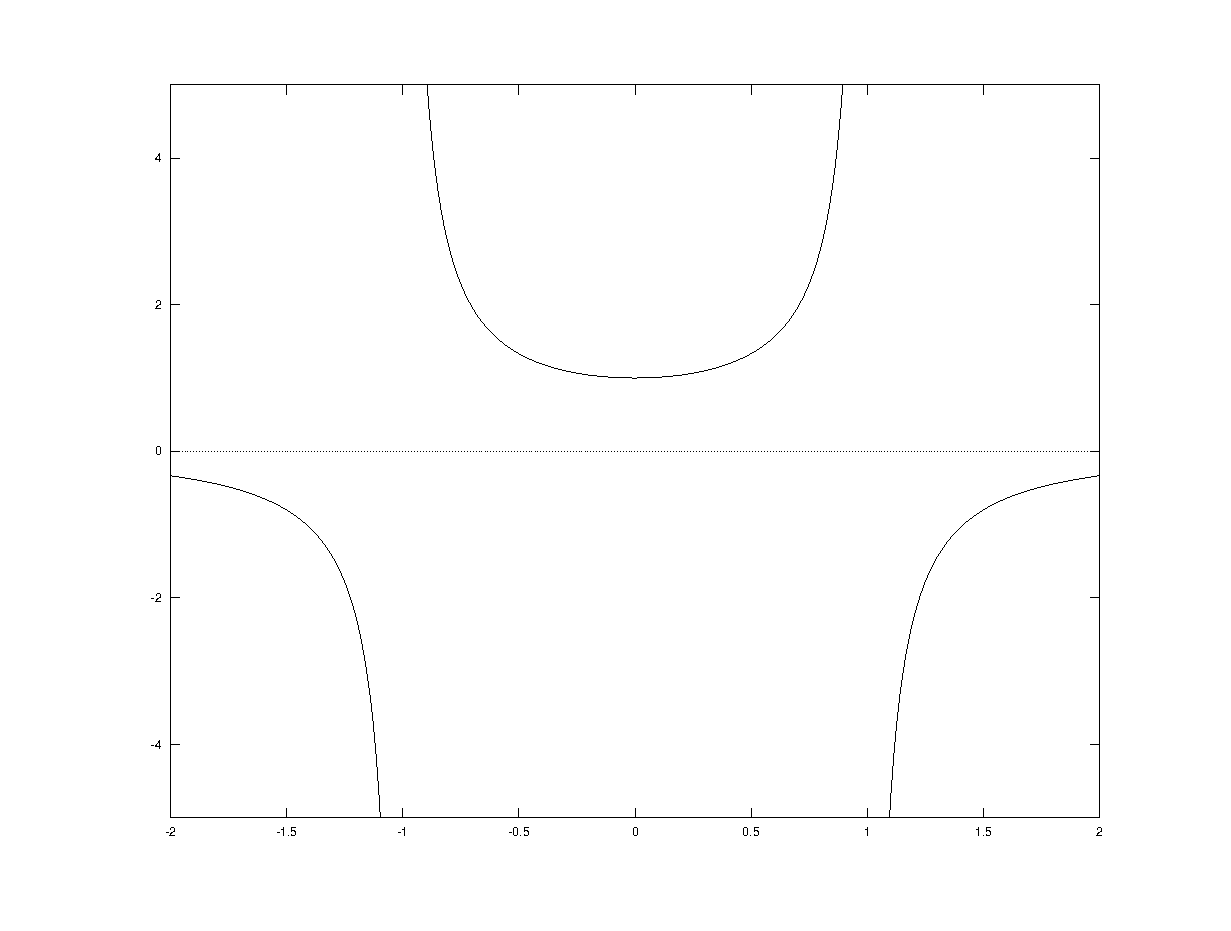
\includegraphics[width=0.8\textwidth]{plot3b.eps}
	\end{center}
	
	\pagebreak
	
	\item[(c)] Graph of $f(x)=\frac{1}{1-x^2}$ with vertical asymptotes.
	\begin{center}
		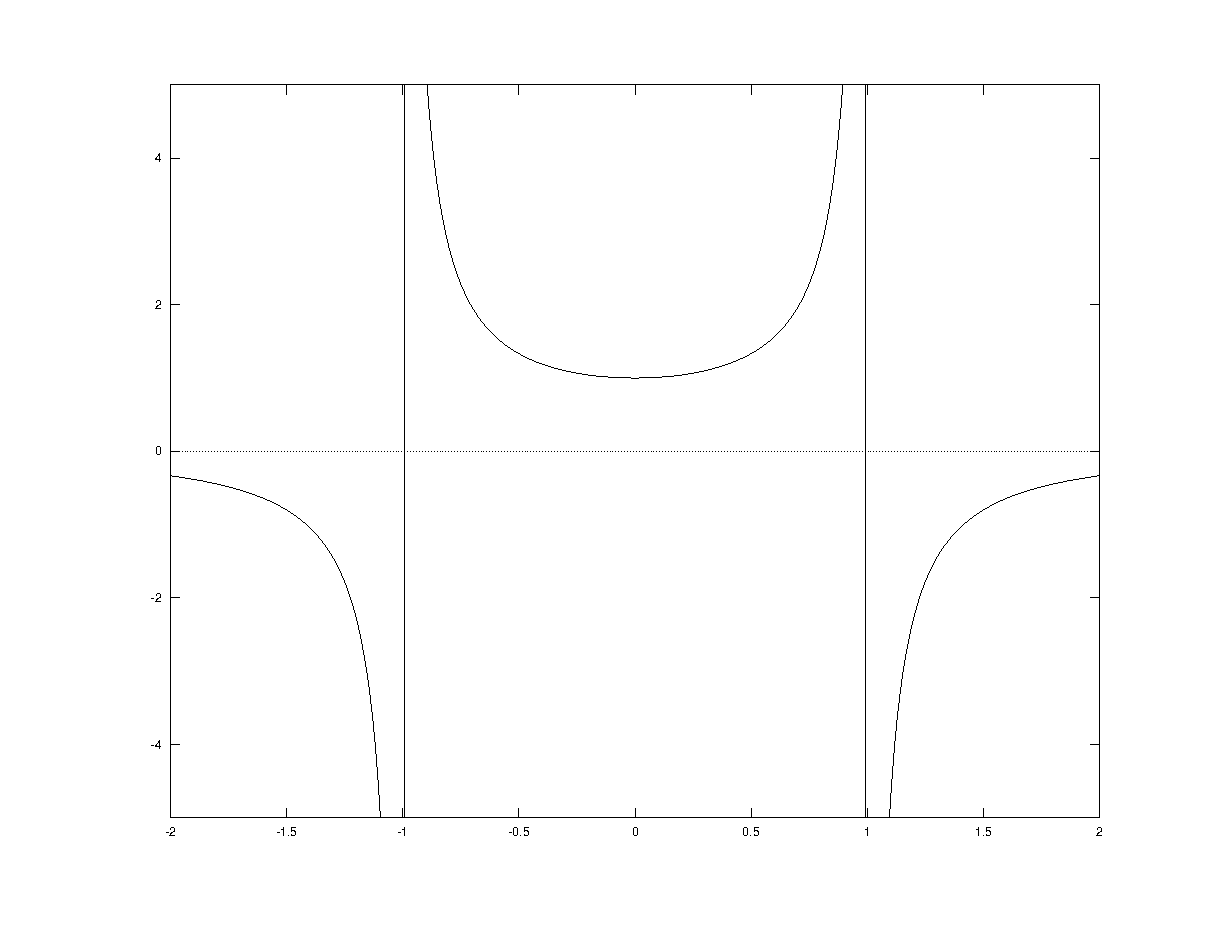
\includegraphics[width=0.8\textwidth]{plot3c.eps}
	\end{center}
	
\end{enumerate}

\subsubsection*{Question 4} 
\begin{enumerate}
	\item[(a)] No
	\item[(b)] No
	\item[(c)] Yes
	\item[(d)] No
\end{enumerate}

\pagebreak

\subsubsection*{Question 5}
\begin{enumerate}
	\item[(a)] Please see Appendix.
	\item[(b)] Central difference approximation (CDA) has a smaller minimum error while forward difference approximation (FDA) has a smaller value of $h$ at which minimum error occurs.
	\item[(c)] Log-log plots of error against $h$ comparing difference approximation methods.
	\begin{center}
		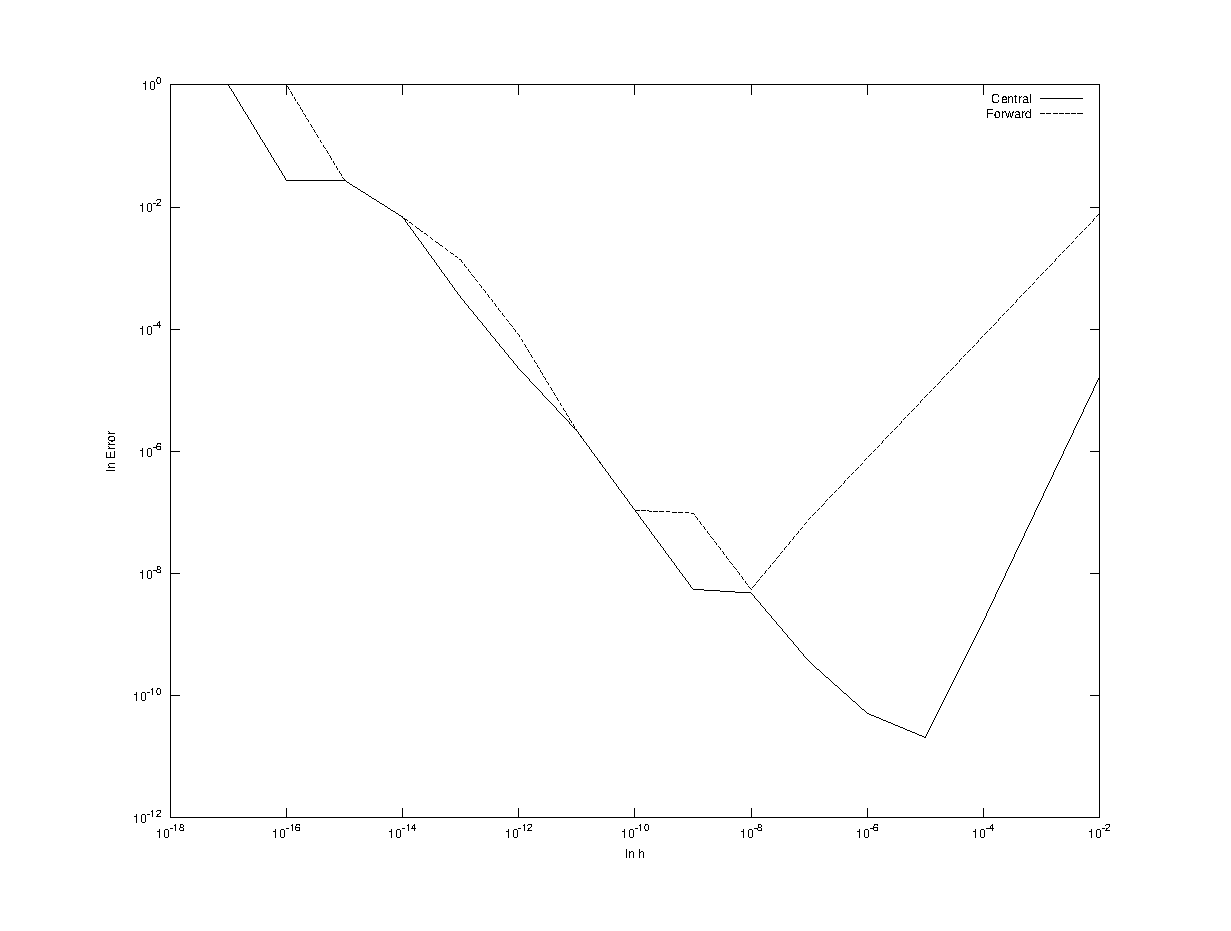
\includegraphics[width=0.9\textwidth]{plot5c.eps}
	\end{center}
	\item[(d)] Truncation error under CDA decreases as $h$ decreases to $10^{-5}$ while FDA's truncation error decreases to even smaller values of $h$, until $10^{-8}$. Cancellation error under CDA begins to increase at $h=10^{-5}$ until $10^{-17}$, while FDA's cancellation error increases from $h=10^{-8}$ until $h=10^{-16}$.
\end{enumerate}
\pagebreak

\subsubsection*{Question 6}
\begin{enumerate}
	\item[(a)] Let $g(x)=e^x-1$ and $h(x)=x$. Since \ $\lim g(x) \ \text{and} \ \lim h(x) \ \text{are both} \ 0$ \ as $x$ approaches 0, then by l'Hopital's Rule
	$$\lim_{x\rightarrow 0} \frac{e^x-1}{x} = \lim_{x\rightarrow 0} \frac{e^x}{1}=e^0=1$$
	\item[(b)] My results do not exactly agree with theoretical expectations since increasing $k$ should improve our approximation's precision by virtue of $x$ approaching 0. However, we see from the graph below that minimum error occurs at $k=8$. For $k>8$, error due to cancellation begins to increase and our approximation worsens as $k$ increases.
	\begin{center}
		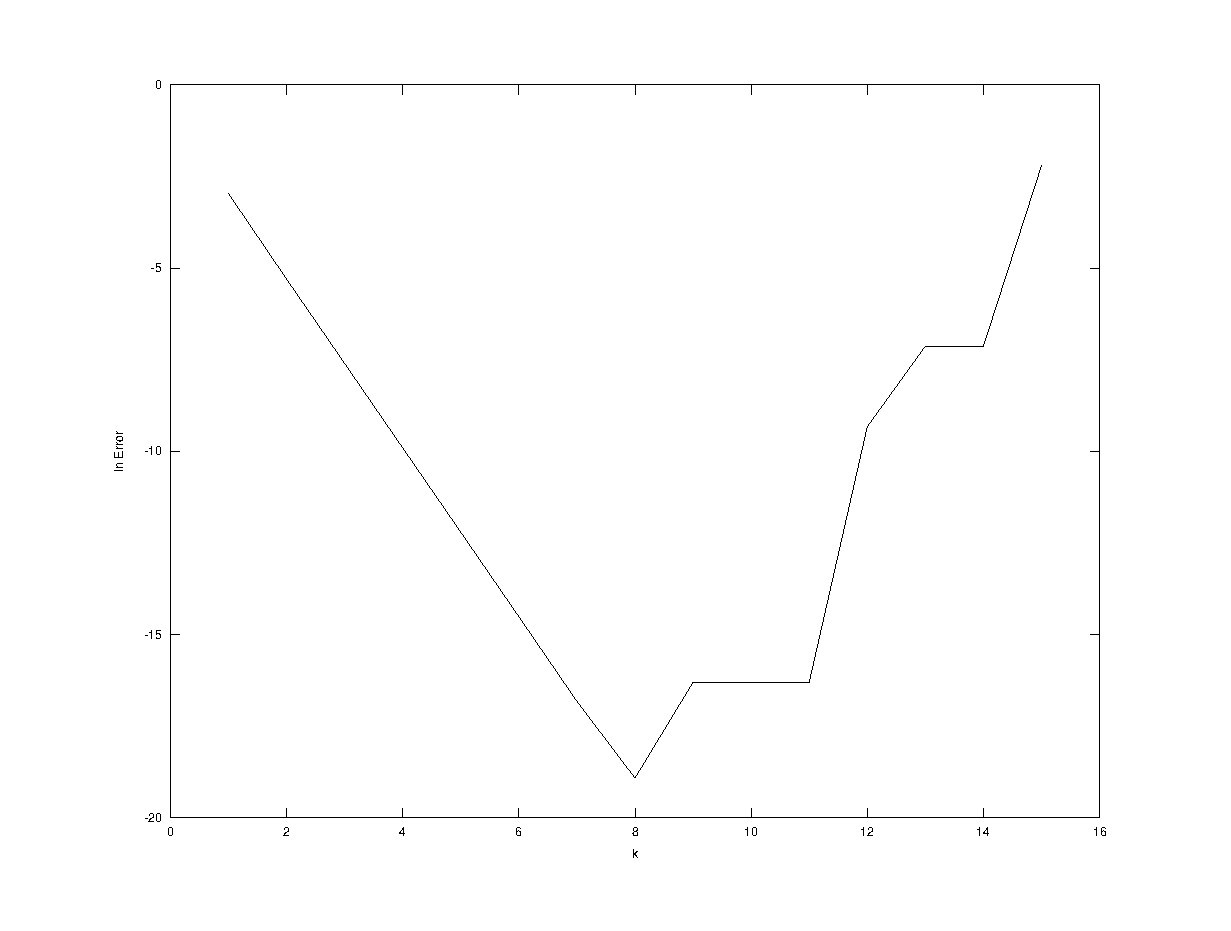
\includegraphics[width=0.9\textwidth]{plot6b.eps}
	\end{center}
\end{enumerate}

\pagebreak

\textbf{Appendix}

\begin{enumerate}
	\item
	\begin{verbatim}
		%graph of f(x)=(x-3)(x-1)
		x1=linspace(0,4,200);
		f1=x1.^2-4*x1+3;
		plot(x1,f1)
		hold on
		xaxis=zeros(1,200);
		plot(x1,xaxis,'.')
		hold on
		x1=1;
		f1=x1.^2-4*x1+3;
		plot(x1,f1,'x')
		hold on
		x1=3;
		f1=x1.^2-4*x1+3;
		plot(x1,f1,'x')
	\end{verbatim}
	
	\item
	\begin{enumerate}
		\item
		\begin{verbatim}
			%graph of f(x)=xlnx
			x2=linspace(0,2,200);
			f2=x2.*log(x2);
			plot(x2,f2)
		\end{verbatim}
	\end{enumerate}
	
	\item
		\begin{enumerate}
		
			\item
			\begin{verbatim}
				%graph of f(x)=1/(1-x^2) with default scaling
				x3=linspace(-2,2,317);
				f3=1./(1-x3.^2);
				plot(x3,f3)
				xaxis=zeros(1,317);
				hold on
				plot(x3,xaxis,'.')
			\end{verbatim}
			
			\item
			\begin{verbatim}
				%graph of f(x)=1/(1-x^2) with rescaled y-axis
				axis([-2,2,-5,5])
			\end{verbatim}
			
			\item
			\begin{verbatim}
				%graph of f(x)=1/(1-x^2) with vertical asymptotes
				figure(2)
				x3=linspace(-2,2,318);
				f3=1./(1-x3.^2);
				plot(x3,f3)
				axis([-2,2,-5,5])
				xaxis=zeros(1,318);
				hold on
				plot(x3,xaxis,'.')
			\end{verbatim}
			
		\end{enumerate}

\pagebreak
			
	\item[5.]
	\begin{enumerate}
		\item
		\begin{verbatim}
			%central difference approximation to f'(x) for f(x)=sin(x) at x=1
			n=-2:-1:-17;
			h=10.^n;
			exact=cos(1);
			approx_c=(sin(1+h)-sin(1-h))./(2*h);
			err_c= abs(approx_c-exact)/exact;
		\end{verbatim}
		
		\item
		\begin{verbatim}
			%forward difference approximation to f'(x) for f(x)=sin(x) at x=1
			approx_f=(sin(1+h)-sin(1))./h;
			err_f= abs(approx_f-exact)/exact;
		\end{verbatim}
		
		\item
		\begin{verbatim}
			%log-log plots of error against h comparing central and
			% forward difference approximation
			loglog(h,err_c,'b',h,err_f,'r')
			xlabel('ln h')
			ylabel('ln Error')
			legend('Central','Forward')
		\end{verbatim}
	\end{enumerate}
	
	\item[6.]
	\begin{enumerate}
		\item[(b)]
		\begin{verbatim}
			%approximates f(x)=(e^x-1)/x for x=10^(-k), k=1,...,15 and graphs
			%its precision errors
			k=1:1:15;
			x=10.^(-k);
			f=(e.^x-1)./x;
			exact=1;
			err=abs(f-exact);
			plot(k,log(err))
			axis([0,16,-20,0])
			xlabel('k')
			ylabel('ln Error')
		\end{verbatim}
	\end{enumerate}
	
\end{enumerate}

\end{document}